\RequirePackage[T1]{fontenc}
\documentclass[conference,letterpaper]{IEEEtran}
\IEEEoverridecommandlockouts
\usepackage{iftex}
\ifPDFTeX
  \usepackage[T1]{fontenc}
  \usepackage{newtxtext,newtxmath}
\else
  \usepackage{newtxtext,newtxmath}
  \AtBeginDocument{\defaultfontfeatures{}\setmainfont{Times New Roman}}
\fi
\usepackage{amsmath}
\usepackage{graphicx}
\usepackage{array,booktabs,tabularx}
\usepackage[super,nomove]{cite}
\usepackage{url}
\usepackage{microtype}
\usepackage[hidelinks]{hyperref}
\graphicspath{{figures/}}
\interdisplaylinepenalty=2500
\setlength{\emergencystretch}{1.2em}
\renewcommand{\figurename}{Figure}
\renewcommand{\tablename}{Table}
\renewcommand{\thetable}{\arabic{table}}
\makeatletter
\def\fnum@figure{Figure~\thefigure}
\def\@citess#1{\mbox{\textsuperscript{\OverciteFont{[#1]}}}}
\renewcommand{\IEEEkeywordsname}{Keywords}
\def\fnum@table{Table~\thetable.}
\makeatother

\title{A Resource-Constrained Network Defense Decision Method Based on a Nonzero-Sum Differential Game}
\author{\IEEEauthorblockN{[First Name Last Name]$^{*}$ \qquad [First Name Last Name]}
\IEEEauthorblockA{[Department / School], [University or Organization]\\
\mbox{[City]}, [Postal Code], [Country]\\
\mbox{[corresponding.author@example.edu]}$^{*}$ \quad [coauthor@example.edu]}}
\begin{document}
\maketitle
\begin{abstract}
To address cross-asset attack propagation and limited defense capacity in multi-asset networks, this paper establishes a complete-information, nonzero-sum, open-loop differential game. Asset-level compromised fractions describe network-state evolution, while isolation and recovery controls specify the defender's resource allocation over time. Continuous-time strategies are parameterized using piecewise-constant controls. By combining fourth-order Runge--Kutta integration, sequential least-squares programming, and alternating best responses, Alternating Best Response for Dynamic Defense Action Decision (ABR-DAD) is developed to calculate isolation and recovery intensities for each asset and time interval. A directed multi-asset propagation network is constructed to examine the spatiotemporal allocation of resources under different defense capacities. Dynamic defense, fixed-mean defense, and no defense are compared in terms of compromised states and cumulative losses under the same time-varying attack sequence. Simulations show that the computed plans satisfy instantaneous capacity constraints and yield differentiated resource allocation. In the main-capacity comparison under the shared attack plan generated with dynamic defense, the dynamic plan reduces cumulative weighted compromise loss and total cumulative defender loss relative to both reference schemes. These results support the method for computing defense schedules under finite resources.
\end{abstract}
\begin{IEEEkeywords}
network defense decision-making, nonzero-sum differential game, alternating best response, attack propagation, resource allocation
\end{IEEEkeywords}

\section{Introduction}
A multi-asset network comprises interrelated logical assets, including entry services, business processing, identity authentication, and core data. Attacks can propagate from entry points to downstream assets along directed paths, causing compromise across multiple assets and business losses. A defender can suppress outgoing propagation through source-side isolation or reduce local compromise through recovery. These actions differ in security effects, business impacts, and resource consumption. Under limited capacity, the defender must account for the attacker's strategy when determining the type, intensity, and timing of defensive actions.

Regarding network propagation control and resource allocation, Preciado \emph{et al.}\cite{r1} studied the allocation of protection resources to inhibit spreading processes in directed networks. Al-Eiadeh and Abdallah\cite{r2} allocated defense resources to interdependent systems using attack graphs and PageRank. Paarporn and Xu\cite{r3} examined resource tradeoffs between preventive and reactive defenses, while Chen \emph{et al.}\cite{r4} investigated the effects of protection and recovery investments and node priorities on network robustness. These studies provide a basis for characterizing propagation structure, asset importance, and defense costs.

In network attack--defense games, Shao and Li\cite{r5} used a multistage attack--defense graph to examine resource allocation during sequential attacks. Hu \emph{et al.}\cite{r6} optimized moving-target defense through a Markov differential game, and Lou \emph{et al.}\cite{r7} studied dynamic collaborative defense in crowdsensing networks under incomplete information. Huang and Zhu\cite{r8} used a susceptible--infected--susceptible (SIS) propagation model and a differential-game framework to study virus suppression and adaptive adjustment of connection weights in complex networks. Mi \emph{et al.}\cite{r9} introduced stochastic disturbances into network attack--defense state evolution and developed a stochastic differential-game model for defense strategy selection. Tian \emph{et al.}\cite{r10} studied a nonzero-sum attack--defense game for malware propagation in cloud environments. Zhang \emph{et al.} investigated real-time defense in scale-free networks\cite{r11} and potential differential-game decisions in complex networks\cite{r12}. Sun \emph{et al.}\cite{r13} incorporated action and timing choices into a time differential game. These works provide methodological foundations for analyzing strategic interactions alongside network-state evolution.

For post-attack repair, Yang \emph{et al.}\cite{r14} employed a differential game to study host repair under advanced persistent threats (APTs). Wang \emph{et al.}\cite{r15} examined APT lateral movement, repair delays, and resource constraints in time-varying networks. Qin \emph{et al.}\cite{r16} studied defense outsourcing under limited budgets through an impulsive differential game. Existing work thus covers propagation control, strategic interaction, and dynamic repair. This study further addresses the joint spatiotemporal allocation of source-side isolation and local recovery in a directed propagation network under attacker strategy responses and finite capacity constraints.

This paper undertakes three tasks: constructing a nonzero-sum, open-loop differential-game model involving directed propagation, source-side isolation, and local recovery; designing ABR-DAD using piecewise-constant controls and alternating best responses to compute defensive actions by asset and interval; and analyzing allocations across defense capacities while comparing dynamic, fixed-mean, and no-defense plans under a common attack sequence in terms of compromised states and cumulative losses.

\section{Multi-Asset Network Attack--Defense Differential-Game Model}
\subsection{Network State}
Represent the multi-asset network as a directed weighted graph $\mathcal{G}=(V,E)$, where $V=\{v_1,\ldots,v_n\}$ is the set of logical assets and $E$ contains attack-propagation edges for which exploitation is feasible. Let $\beta_{ji}\geq0$ be the effective propagation rate from source asset $j$ to target asset $i$, with $\beta_{ji}=0$ when no edge exists and $\beta_{ii}=0$. Let $x_i(t)\in[0,1]$ denote the compromised fraction of the workload-instance group corresponding to asset $i$ at time $t$. It is an aggregate measure of compromise among instances of the same workload type and describes the network state.

The attacker allocates entry attack intensity $a_i(t)$ only to the entry-index set $I_A\subseteq\{1,\ldots,n\}$; for non-entry assets $a_i(t)=0$. The defender chooses source-side isolation $s_i(t)$ and local recovery $r_i(t)$. All three controls have normalized intensities in $[0,1]$. Define the total compromise pressure on asset $i$ at time $t$ as
\begin{equation}\label{eq:pressure}
\lambda_i=\alpha_i a_i+\sum_{j\ne i}\beta_{ji}(1-\varepsilon_j s_j)x_j.
\end{equation}
The compromised-state dynamics are
\begin{equation}\label{eq:state}
\dot x_i=(1-x_i)\lambda_i-(\delta_i+\gamma_i r_i)x_i.
\end{equation}
Here $\alpha_i$ is direct attack efficiency ($0$ for non-entry assets), $\varepsilon_j$ is source-isolation efficiency, $\delta_i$ is the baseline recovery rate, $\gamma_i$ is recovery effectiveness coefficient, and $x_i(0)=x_{i0}$. In \eqref{eq:pressure}, $s_j$ only reduces outgoing propagation from source $j$. In \eqref{eq:state}, $r_i$ directly reduces the compromised fraction of asset $i$ and indirectly suppresses subsequent propagation through state evolution. For finite nonnegative model parameters, bounded controls, and $0\leq\varepsilon_js_j\leq1$, the state set $[0,1]^n$ is positively invariant. Given an initial state and control plans, the state system has a unique trajectory over the finite horizon, providing a deterministic state mapping for numerical evaluation of both objectives.

Isolation acts on outgoing propagation from a source asset, whereas recovery reduces local compromise. Their effectiveness depends on propagation links, compromised states, and the remaining planning horizon.

\subsection{Game Model}
A complete-information, two-player, noncooperative, nonzero-sum, open-loop differential game is defined on the continuous-time state system. At the planning origin, both players know the network topology, initial state, model parameters, objective functions, and constraints, and separately choose open-loop control plans over the horizon.

\emph{Definition 1 (Multi-asset network attack--defense differential game).} The game comprises players, a planning horizon, strategy sets, network state, state-transition function, and objective functions, written as the six-tuple $\Gamma=(\mathcal N,\mathcal T,\mathcal P,x,f,\mathcal J)$:

\emph{1) Players:} $\mathcal N=\{N_D,N_A\}$. The defender selects isolation and recovery, while the attacker selects entry attack intensities; each evaluates strategies according to its own objective.

\emph{2) Horizon:} $\mathcal T=[0,T]$, where $T>0$ is the terminal time and horizon length. At $t=0$, the players specify open-loop plans over $\mathcal T$. Controls may vary in time while the network state evolves continuously.

\emph{3) Strategy sets:} $\mathcal P=(\mathcal U,\mathcal A)$, where $\mathcal U$ and $\mathcal A$ are the feasible defender and attacker open-loop strategy sets satisfying control bounds, entry restrictions, and capacity constraints. The defender's plan comprises time-varying isolation and recovery controls.

\emph{4) State:} $x(t)\in[0,1]^n$ is the vector of compromised fractions for all assets, jointly determined by attack inputs, defensive actions, and propagation.

\emph{5) State transition:} $\dot x(t)=f(t,x(t),u(t),a(t))$ is specified by \eqref{eq:pressure}--\eqref{eq:state} and describes continuous compromise evolution and cross-asset dependencies.

\emph{6) Objectives:} $\mathcal J=(J_D,J_A)$ comprises the defender's total cumulative loss and the attacker's cumulative net payoff, with distinct state weights and action costs.

The defender minimizes asset-compromise loss, business impact from isolation, and control costs. Its instantaneous total loss is decomposed as
\begin{equation}\label{eq:ellD}
\ell_D=\sum_{i=1}^n(q_i x_i+h_i s_i)+C_D,
\end{equation}
\begin{equation}\label{eq:CD}
C_D=\frac12\sum_{i=1}^n(c_i^s s_i^2+c_i^r r_i^2).
\end{equation}
The attacker maximizes the net payoff obtained by subtracting attack costs from compromise gains:
\begin{equation}\label{eq:ellA}
\ell_A=\sum_{i=1}^n g_i x_i-C_A,
\end{equation}
\begin{equation}\label{eq:CA}
C_A=\frac12\sum_{i=1}^n c_i^a a_i^2.
\end{equation}
Over the finite horizon $[0,T]$, the two objectives are
\begin{equation}\label{eq:JD}
J_D(u,a)=\int_0^T\ell_D\,dt+\omega^{\mathsf T}x(T),
\end{equation}
\begin{equation}\label{eq:JA}
J_A(u,a)=\int_0^T\ell_A\,dt+\nu^{\mathsf T}x(T).
\end{equation}
Here $u=(s,r)$; $q_i$ and $g_i$ are the defender's compromise-loss and the attacker's compromise-payoff weights, respectively; $h_i$ represents isolation-induced business impact; $c_i^s,c_i^r,c_i^a$ are positive quadratic cost coefficients; and $\omega,\nu$ are terminal-state weights. The defender solves $\min J_D$ and the attacker solves $\max J_A$. Their distinct state weights and action costs produce a nonzero-sum structure, $J_A\ne-J_D$. Isolation inhibits propagation but incurs business impact; recovery reduces local compromise while incurring control cost. The attacker balances compromise payoff against attack cost. The two objectives are not negatives of each other.

Let $B_D$ and $B_A$ denote the defender's and attacker's instantaneous resource capacities, respectively. At each time,
\begin{equation}\label{eq:BD}
\sum_i (b_i^s s_i+b_i^r r_i)\leq B_D,
\end{equation}
\begin{equation}\label{eq:BA}
\sum_{i\in I_A}d_i^a a_i\leq B_A.
\end{equation}
The bounds are $0\le a_i,s_i,r_i\le1$ with $a_i=0$ for non-entry assets. The coefficients $b_i^s,b_i^r,d_i^a$ give capacity consumption per unit control intensity. Equations \eqref{eq:BD}--\eqref{eq:BA} constrain simultaneous resource inputs, whereas \eqref{eq:CD} and \eqref{eq:CA} describe time-accumulated control costs. The model uses normalized relative units; experimental control intensities represent resource allocation at the model level.

Instantaneous capacity limits simultaneous inputs, while business impact and quadratic control costs accumulate over time. Consequently, the defender need not exhaust capacity in every interval. Under Definition 1, the players optimize entire-horizon plans over their known information and feasible strategies. Dynamic noncooperative game theory\cite{r17} supplies a criterion for their rational strategic relationship.

\emph{Definition 2 (Open-loop Nash equilibrium).} A feasible pair $(u^\star,a^\star)\in\mathcal U\times\mathcal A$ is an open-loop Nash equilibrium when each plan is a best response to the other:
\begin{equation}\label{eq:NEd}
J_D(u^\star,a^\star)\le J_D(v,a^\star),\quad \forall v\in\mathcal U,
\end{equation}
\begin{equation}\label{eq:NEa}
J_A(u^\star,a^\star)\ge J_A(u^\star,b),\quad \forall b\in\mathcal A.
\end{equation}
Equations \eqref{eq:NEd}--\eqref{eq:NEa} define the open-loop Nash equilibrium through mutual best responses. This paper computes numerical responses within a piecewise-constant strategy class to obtain defensive actions for each asset and interval under capacity constraints.

\section{Dynamic Defense Action Computation}
\subsection{Piecewise-Constant Controls and Numerical Best Responses}
Using control parameterization\cite{r18}, divide $[0,T]$ uniformly into $K$ intervals with length $\Delta t=T/K$. For $k=1,\ldots,K$, let $a_{i,k}$, $s_{i,k}$, and $r_{i,k}$ remain constant over interval $k$, while $x(t)$ evolves continuously according to \eqref{eq:state}. Denote the finite-dimensional decision variables by $z_D=\{s_{i,k},r_{i,k}\}$ and $z_A=\{a_{i,k}\mid i\in I_A\}$, with feasible sets $U_K$ and $A_K$.

Holding the opponent's plan fixed, the theoretical best responses within these restricted strategy classes are
\begin{equation}\label{eq:BRD}
BR_D(z_A)=\underset{v\in U_K}{\arg\min}\ J_D(v,z_A),
\end{equation}
\begin{equation}\label{eq:BRA}
BR_A(z_D)=\underset{b\in A_K}{\arg\max}\ J_A(z_D,b).
\end{equation}
Here $v$ and $b$ are candidate defender and attacker plans, and $J_D$ and $J_A$ are the cumulative loss and net payoff defined in Section II. Equations \eqref{eq:BRD}--\eqref{eq:BRA} describe each player's best response to a fixed opponent plan and form the basis of alternating optimization. Fourth-order Runge--Kutta (RK4) integration\cite{r19} evaluates candidate plans; sequential least-squares programming (SLSQP) computes local numerical responses under control bounds and linear capacity constraints\cite{r20,r21}. These local responses are numerical approximations to the theoretical best-response problems in \eqref{eq:BRD}--\eqref{eq:BRA}. The plans are then updated alternately. The final strategies undergo deviation searches from multiple initializations, constraint checks, and integration-refinement tests. The state equation evaluates compromise evolution under a control plan, while the finite-dimensional controls correspond directly to the defense locations, intervals, and intensities that the defender must determine.

\subsection{ABR-DAD Defense Action Computation}
Based on the best-response principle for dynamic noncooperative games\cite{r17} and related iterative work\cite{r22}, we design Alternating Best Response for Dynamic Defense Action Decision (ABR-DAD). Its purpose is to produce a defense action plan: holding the attack plan fixed, optimize isolation and recovery; then, holding the defense plan fixed, compute the attack response; and alternate until the numerical stopping conditions are met. The procedure is shown in Algorithm 1.

\begin{figure}[t]
\centering
\begin{minipage}{\columnwidth}
\hrule\vspace{2pt}
{\footnotesize\textbf{Algorithm 1.} Alternating Best Response for Dynamic Defense Action Decision (ABR-DAD)}\par\vspace{2pt}
{\footnotesize
\textbf{Input:} $\mathcal G,x_0,T,K,B_D,B_A$, model parameters $\theta$, stopping tolerances $\epsilon$, iteration bound $M$.\par
\textbf{Output:} actions $D$, resource use $R$, final player plans, $J_D$, diagnostics.\par
1. Initialize capacity-feasible $z_D^{(0)},z_A^{(0)}$.\par
2. \textbf{for} $m=0,1,\ldots,M-1$ \textbf{do}\par
3. \quad Fix $z_A^{(m)}$; obtain local defender response $z_D^{(m+1)}$ with RK4 and SLSQP.\par
4. \quad Fix $z_D^{(m+1)}$; obtain local attacker response $z_A^{(m+1)}$ with RK4 and SLSQP.\par
5. \quad Check single-start unilateral deviations and compute $gap_D,gap_A$.\par
6. \quad Compute stationarity residual $stat$, response distance $dist$, and capacity violation $viol$.\par
7. \quad \textbf{if} both SLSQP runs exit normally and all three stopping metrics pass \textbf{then break}.\par
8. \textbf{end for}\par
9. Run three-start deviation checks, refine integration, recompute trajectories, and form $D_{i,k},R_{i,k}$.\par
10. \textbf{return} $D,R$, final plans, $J_D$, and diagnostics.
}\vspace{3pt}\hrule
\end{minipage}
\end{figure}

The maximum number of alternating iterations is $M=40$; each SLSQP solve allows at most 300 iterations with a tolerance of $10^{-10}$. Complete alternating runs start from uniform feasible, zero-control, and random feasible plans, while each individual player optimization uses the current plan as its sole starting point. The stopping metrics are normalized discovered unilateral improvement $\eta_p$, projected-gradient stationarity residual $stat_p$, and response distance $dist_p$, where $\eta_p=gap_p/(1+|J_p|)$ for $p\in\{D,A\}$. Once both SLSQP solvers exit normally, stopping is declared if the maxima of the three metrics across both players do not exceed $10^{-7}$, $10^{-4}$, and $10^{-3}$, respectively. 

For the stopping diagnostics, write $F_D=J_D$ and $F_A=-J_A$, with the opponent's plan fixed. Let $\widetilde z_p$ be the numerical unilateral response and let $\mathcal F_D=U_K$ and $\mathcal F_A=A_K$. The discovered improvement is $gap_p=\max\{0,F_p(z_p)-F_p(\widetilde z_p)\}$. We use the unit-step projected-gradient residual $stat_p=\|z_p-\Pi_{\mathcal F_p}(z_p-\nabla F_p(z_p))\|_\infty$ and the response distance $dist_p=\|\widetilde z_p-z_p\|_\infty$, where $\Pi$ is Euclidean projection onto the bounded, capacity-constrained feasible set. Response candidates are accepted only if their bound and capacity violations are at most $10^{-10}$. The single-start checks used for stopping are distinct from the three-start searches performed after termination.

The defender then obtains an isolation and recovery plan by asset and interval. For asset $i$ and interval $k$,
\begin{equation}\label{eq:action}
D_{i,k}=(s_{i,k},r_{i,k}),
\end{equation}
\begin{equation}\label{eq:R}
R_{i,k}=b_i^s s_{i,k}+b_i^r r_{i,k}.
\end{equation}
Equations \eqref{eq:action}--\eqref{eq:R} specify where, when, and at what intensities isolation and recovery are applied, while guaranteeing $\sum_i R_{i,k}\le B_D$. After iteration, each final player plan is held fixed in multiple-start deviation searches. Capacity, local stationarity, and integration consistency are checked, and the actions, state trajectories, and cumulative losses of all assets and intervals are saved for reproducibility.

After alternating best-response iterations, the numerical response consistency of the final strategies is examined. With one final plan held fixed, the other player is allowed to search again over feasible strategies to determine whether a unilateral adjustment can improve its own objective. Construct finite candidate sets $\mathcal C_D\subseteq U_K$ and $\mathcal C_A\subseteq A_K$ through multiple-start deviation searches and calculate discovered unilateral improvements:
\begin{equation}\label{eq:gapD}
\widehat\Delta_D=J_D(z_D,z_A)-\min_{v\in\mathcal C_D}J_D(v,z_A),
\end{equation}
\begin{equation}\label{eq:gapA}
\widehat\Delta_A=\max_{b\in\mathcal C_A}J_A(z_D,b)-J_A(z_D,z_A).
\end{equation}
Here $z_D,z_A$ are the final plans and $v,b$ are candidate deviations. Equations \eqref{eq:gapD}--\eqref{eq:gapA} test whether, with the opponent's final plan fixed, the defender can further reduce comprehensive loss or the attacker can increase net payoff. Since each candidate set includes the current plan, both discovered unilateral improvements are nonnegative. A zero improvement means that no better unilateral plan was found within the finite candidate search range.

\subsection{Convergence and Interpretation of the Computed Plans}
ABR-DAD computes a candidate strategy pair in $U_K\times A_K$. Three distinctions govern its interpretation. First, the piecewise-constant parameterization restricts the admissible deviations. Second, SLSQP returns local numerical responses and does not certify global solutions of the restricted best-response problems. Third, alternating responses in a general nonzero-sum game need not converge: one player's update can change the other player's objective unfavorably, and neither objective is a common descent function. Cycling or failure to meet the stopping tolerances is therefore possible. The iteration limit bounds computational effort; reaching it alone does not establish response consistency.

If exact global best responses converge to a mutually optimal pair, that pair is a Nash equilibrium of the restricted game. The local solves and finite deviation searches used here do not establish this premise. The discovered improvements in \eqref{eq:gapD}--\eqref{eq:gapA} are lower bounds on the maximum unilateral improvements within the restricted strategy sets, rather than certified upper error bounds. Small values, together with stationarity and response-distance checks, provide numerical evidence for the reported candidate, without certifying an $\epsilon$-Nash equilibrium or a continuous-time equilibrium. Multiple initializations assess observed sensitivity; integration refinement checks trajectory evaluation for fixed controls, not convergence with respect to $K$.

\section{Simulation Experiments and Results}
\subsection{Experimental Setup}
A directed multi-asset attack-propagation network is constructed as shown in Figure~\ref{fig:network}. The nodes are $v_1$: application programming interface (API) gateway, $v_2$: Web application, $v_3$: order processing, $v_4$: identity authentication, $v_5$: core database, and $v_6$: back-end management. Nodes $v_1$ and $v_2$ are direct attack entry points; $v_4$ has multiple outgoing propagation edges, and $v_5$ has a high loss weight but no outgoing propagation. The effective edges and rates are $1\!\to\!3$: 0.08, $1\!\to\!4$: 0.09, $2\!\to\!3$: 0.10, $4\!\to\!3$: 0.11, $4\!\to\!5$: 0.07, $4\!\to\!6$: 0.12, $3\!\to\!5$: 0.10, and $6\!\to\!5$: 0.05. This is a synthetic six-asset network with preset propagation parameters and normalized time, control intensities, and costs. Table~\ref{tab:params} summarizes the simulation parameters.

\begin{figure}[t]
\centering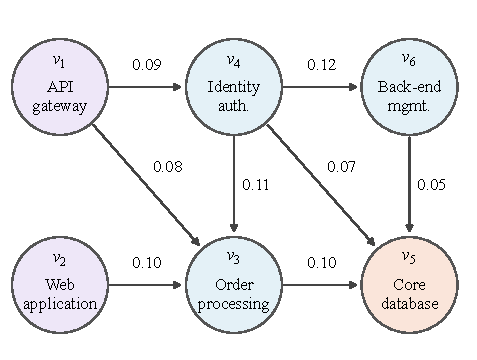
\includegraphics[width=3.18in]{fig1_network_en.pdf}
\caption{Directed attack-propagation network with multiple assets.}\label{fig:network}
\end{figure}

\begin{table}[t]
\caption{Main simulation parameters.}\label{tab:params}
\centering\footnotesize
\renewcommand{\arraystretch}{1.11}
\begin{tabularx}{\columnwidth}{@{}p{.30\columnwidth}X@{}}\toprule
Category & Parameter values \\ \midrule
Network and horizon & $n=6$, $T=10$, $K=6$, $\Delta t=5/3$\\
Initial state and attack capacity & $x(0)=(0.1,0,0,0,0,0)$; $B_A=0.8$\\
Defense capacity & $B_D\in\{0.6,1.2,1.8\}$; main case $B_D=1.2$\\
Direct attack and isolation & $\alpha_1=\alpha_2=0.25$, other $\alpha_i=0$; $\varepsilon_i=1$\\
Recovery and weights & $\delta_i=0.1$, $\gamma_i=0.3$; $q=(1,1,1,1,4,1)$, $g_i=1$\\
Costs, capacity, terminal weights & $h_i=0.05$, $c_i^s=c_i^r=c_i^a=1$; $b_i^s=b_i^r=d_i^a=1$; $\omega=\nu=0$\\
\bottomrule\end{tabularx}
\end{table}

For main capacity $B_D=1.2$, dynamic defense (G), fixed-mean defense (M), and no defense (N) are compared under the attack-control trajectory computed jointly with G and then held fixed for all three schemes. G is the six-interval isolation and recovery plan computed by ABR-DAD. M keeps each of the two controls for each asset constant at its arithmetic mean over the six intervals, while N sets isolation and recovery to zero. G and M have equal cumulative input for each asset and action type and both satisfy the instantaneous capacity constraint. Network topology, initial state, attack sequence, and model parameters are identical; only the defense plans change, allowing comparison of executed defense outcomes under a shared attack input. State trajectories and cumulative losses are computed from the model in Section II, using 48 RK4 substeps per control interval. Capacities $B_D=0.6$ and $1.8$ are used to illustrate resource allocation under varying capacity.

The archived optimization used Python 3.11.7, NumPy 1.26.4, and SciPy 1.11.4 on Windows. The base random seeds were 20262114, 20261114, and 20263114 for capacities 0.6, 1.2, and 1.8, respectively; the random full-run initialization used the corresponding base seed plus two. The uniform-start plan was selected for reporting. Saved controls, trajectories, diagnostic records, and figure-generation inputs accompany the manuscript source.

All three uniform-start paths first met the stopping criteria after five alternating updates. At updates 3 and 4, discovered-improvement and response-distance thresholds were already met in all three paths, whereas the current-plan stationarity residual remained above its threshold. Thus, in these archived runs the residual check prevented stopping before the stated stationarity tolerance was satisfied; this observation is not an ablation study. Across the three capacities and both players, the normalized discovered improvement, current-plan projected residual, and response distance did not exceed \mbox{$2.90\times10^{-10}$}, \mbox{$6.48\times10^{-5}$}, and \mbox{$3.35\times10^{-5}$}, respectively; all final single-start SLSQP exit codes were zero. The largest control difference between full-run initializations was below \mbox{$4.02\times10^{-5}$}. Separate three-start checks of the final reported plans also passed the stated local criteria. For the three main-capacity comparison plans, increasing RK4 substeps per control interval from 48 to 192 changed shared-time states by at most \mbox{$8.71\times10^{-12}$}. These archived runs demonstrate satisfaction of the numerical stopping criteria in the tested cases, rather than a general convergence guarantee.

\subsection{Defense Resource Allocation}
The experiment first reports the defender's resource inputs and concrete actions across control intervals to assess whether the method produces capacity-feasible defense schedules across assets and time intervals. Under $B_D=1.2$, G uses capacities 0.843705, 1.200000, 1.200000, 1.200000, 1.065570, and 0.337751 in the six intervals. The capacity bound is active in intervals 2--4 and slack in the others. With $B_D=0.6$, capacity is fully used in the first five intervals; with $B_D=1.8$, all intervals retain slack, as shown in Figure~\ref{fig:capacity}. Input decreases in the last interval under all three capacities, reflecting the tradeoff between finite-horizon protection benefits and action costs. Accordingly, the defender allocates capacity in view of state evolution and action costs rather than applying fixed-proportion static allocation; the plan exhibits both binding capacity constraints and reduced late-horizon control effort.

\begin{figure*}[!t]
\centering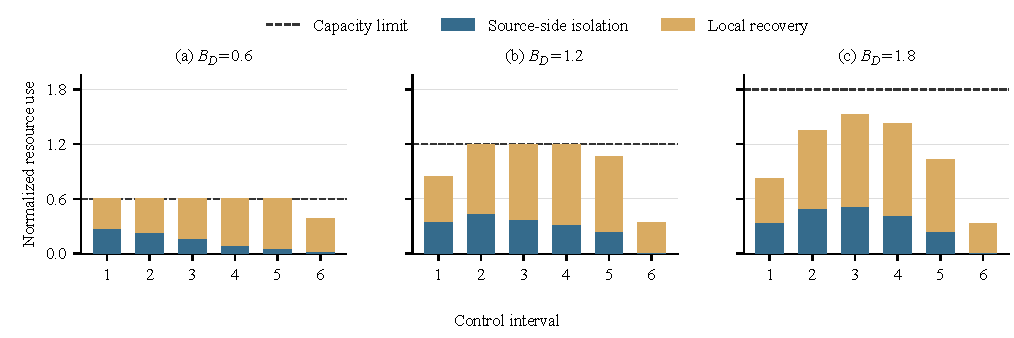
\includegraphics[width=6.76in]{fig2_capacity_en.pdf}
\caption{Resource use by control interval under three defense capacities.}\label{fig:capacity}
\end{figure*}

\begin{table}[t]
\caption{Mean defensive resource use per asset under three capacities.}\label{tab:asset}
\centering\footnotesize\renewcommand{\arraystretch}{1.13}
\begin{tabular}{@{}lrrr@{}}\toprule
Asset & $B_D=0.6$ & $B_D=1.2$ & $B_D=1.8$\\\midrule
$v_1$ API gateway & 0.339102 & 0.463738 & 0.480837\\
$v_2$ Web application & 0.116986 & 0.225360 & 0.249486\\
$v_3$ Order processing & 0.056986 & 0.140469 & 0.162958\\
$v_4$ Identity auth. & 0.012188 & 0.076786 & 0.101903\\
$v_5$ Core database & 0.037143 & 0.062960 & 0.073916\\
$v_6$ Back-end mgmt. & 0.001960 & 0.005190 & 0.011925\\\midrule
Total (time mean) & 0.564365 & 0.974504 & 1.081025\\\bottomrule
\end{tabular}
\par\vspace{2pt}{\footnotesize Totals are computed before rounding.}
\end{table}

Table~\ref{tab:asset} presents mean allocations by asset under different capacities. As defense capacity increases, the absolute input to the API gateway grows but its share of total network resources declines; both the input and share of identity authentication increase. Thus, defense resources expand from a relative concentration on entry assets to other assets with propagation influence, indicating dynamic adjustment across assets under finite resources. Figure~\ref{fig:capacity} captures interval-level capacity use, whereas Table~\ref{tab:asset} reports asset-level allocation. Figure~\ref{fig:actions} shows isolation and recovery intensities for six assets over six intervals at $B_D=1.2$, totaling 72 defense-control components, and explicitly identifies action locations, types, and intensities.

\begin{figure*}[!t]
\centering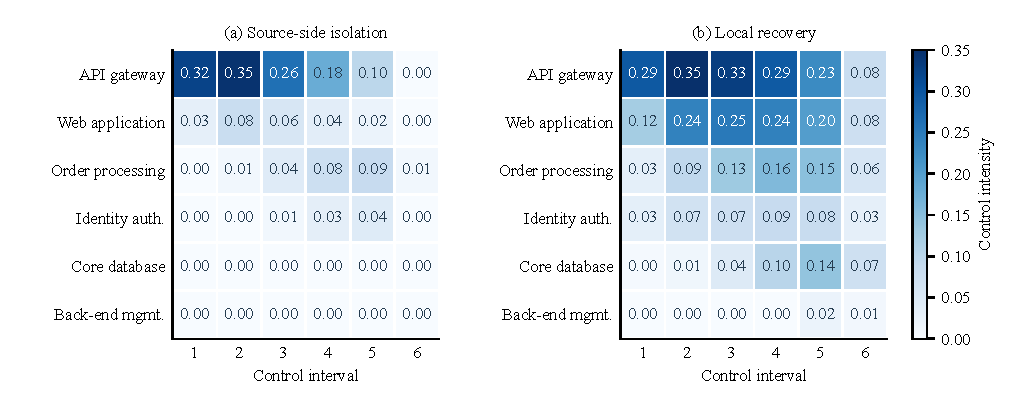
\includegraphics[width=6.76in]{fig3_actions_en.pdf}
\caption{Isolation and recovery actions by asset and interval at the main defense capacity $B_D=1.2$.}\label{fig:actions}
\end{figure*}

The API gateway serves as an attack entry point and connects to order processing and identity authentication, so isolation and recovery are applied together in early intervals. Identity authentication has considerable outgoing propagation influence; its isolation intensity rises in intervals 3--5 and declines in the final interval. The core database has a high loss weight but no outgoing edges and primarily receives local recovery. These allocations accord with the assets' propagation positions and the defensive mechanisms.

\subsection{Evaluation of Defense Effectiveness}
Under the common attack input defined in Section IV-A, three complementary metrics assess the execution outcomes of dynamic, fixed-mean, and no-defense schemes.

\emph{1) Cumulative weighted compromise loss:} $L_{\mathrm{sec}}=\int_0^T\sum_{i=1}^6q_i x_i(t)\,dt$, where $q_i$ is the asset-value weight and $x_i(t)$ is its compromised fraction. The integral reflects both compromise severity and duration.

\emph{2) Total cumulative defender loss:} $J_D=L_{\mathrm{sec}}+C_{ba}$, where $C_{ba}$ is the time integral of the isolation-induced business-impact term in \eqref{eq:ellD} and the quadratic action costs in \eqref{eq:CD}. Since the terminal-state weight is zero in this experiment, the metric equals the defender's objective in Section II and accounts for both security losses and defense costs.

\emph{3) Terminal network value-weighted compromised fraction:} $X_q(T)=\frac{\sum_{i=1}^6 q_i x_i(T)}{\sum_{i=1}^6q_i}$. This metric captures the terminal network condition, distinct from the two cumulative-loss metrics. Together with key-asset trajectories, it characterizes asset protection.

Figure~\ref{fig:states} shows the API gateway, identity authentication, core database, and network value-weighted compromised fractions under the same attack sequence; Table~\ref{tab:effects} summarizes the metrics. At the beginning of interval 6 ($t\approx8.33$), gateway entry attack intensity declines from 0.384142 to 0.139831 and Web entry intensity from 0.365943 to 0.137174. Under all three schemes, the compromise inflow $(1-x_1)\lambda_1$ falls below the recovery outflow $(\delta_1+\gamma_1r_1)x_1$, so the gateway compromised fraction changes from increasing to decreasing. Identity authentication and the core database remain affected by upstream propagation and continue to accumulate compromise, illustrating propagation lag.

Dynamic defense allocates more isolation and recovery to the gateway during early and middle intervals, reducing accumulated compromise earlier. In the final interval, its gateway recovery intensity is 0.080739, below approximately 0.262580 for fixed-mean defense. Consequently, the gateway compromised fraction decreases faster under the fixed scheme and becomes lower than under the dynamic scheme after $t\approx8.49$. A late crossover also occurs for identity authentication, whereas the core database maintains a lower compromised fraction under dynamic defense. The network value-weighted compromised fraction is lower under dynamic defense during most of the horizon, but slightly lower under fixed defense at the terminal time. Cumulative loss and terminal state must therefore be distinguished.

\begin{figure*}[!t]
\centering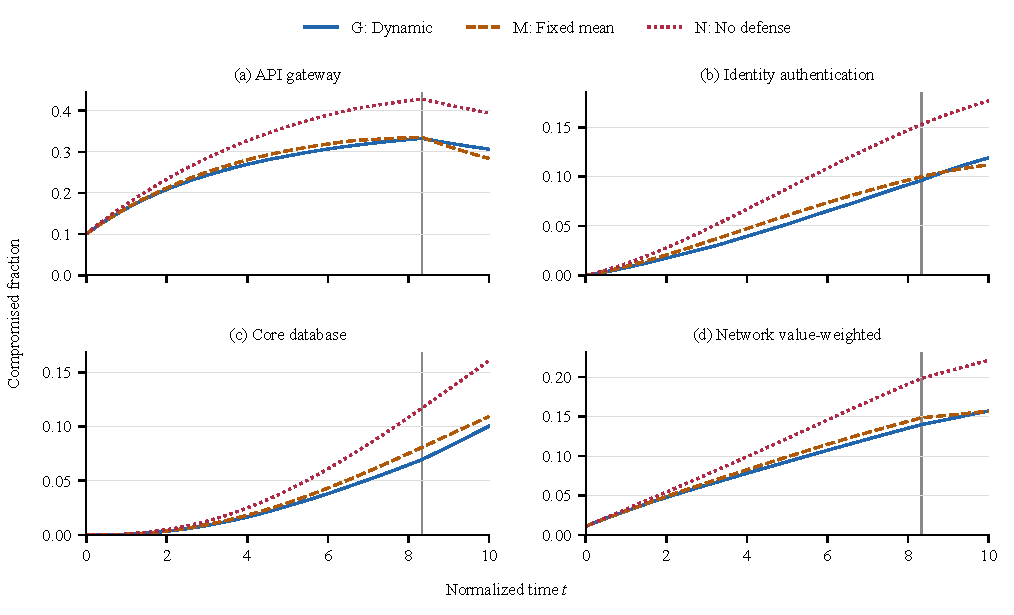
\includegraphics[width=6.76in]{fig4_states_en.pdf}
\caption{Compromised states of key assets and the network under three defense schemes with a common attack sequence ($B_D=1.2$).}\label{fig:states}
\end{figure*}

\begin{table}[!t]
\caption{Three effectiveness metrics and business/action costs under the main defense capacity ($B_D=1.2$).}\label{tab:effects}
\centering\footnotesize\renewcommand{\arraystretch}{1.06}
\setlength{\tabcolsep}{3pt}
\begin{tabularx}{\columnwidth}{@{}Xrrr@{}}\toprule
Metric & N & M & G \\\midrule
Cumulative weighted compromise loss & 10.945701 & 8.580319 & 8.176990\\
Business and action cost & 0.000000 & 0.976515 & 1.149657\\
Total cumulative defender loss & 10.945701 & 9.556834 & 9.326647\\
Terminal weighted compromised fraction & 0.221271 & 0.156868 & 0.157163\\\bottomrule
\end{tabularx}
\end{table}

Table~\ref{tab:effects} reports total cumulative defender losses of 10.945701, 9.556834, and 9.326647 for no defense, fixed-mean defense, and dynamic defense, respectively. The dynamic scheme reduces this loss by approximately 14.79\% and 2.41\% relative to the two alternatives. Under the same attack sequence and equal per-asset cumulative control inputs, adjusting the timing of isolation and recovery reduces cumulative weighted compromise loss by 0.403329 relative to fixed-mean defense. Although the dynamic scheme incurs greater business and action costs and a slightly higher terminal network weighted compromised fraction than fixed-mean defense, its reduction of early accumulated compromise produces a lower total cumulative loss. Hence, the timing of defense actions substantially influences network-state evolution and cumulative protection effectiveness.

At the terminal time, the fixed scheme has a slightly lower network weighted compromised fraction than the dynamic scheme, and both improve on no defense. Figure~\ref{fig:states} also shows that dynamic defense better protects the core database at the terminal time, whereas fixed defense yields lower terminal compromised fractions at the API gateway and identity authentication. Thus, terminal compromise and cumulative loss reflect distinct evaluation dimensions. Overall, the computed dynamic plan reduces cumulative compromise and total defender losses by appropriately timing its actions, without implying minimum compromise for every asset at every instant.

\subsection{Model Applicability}
The complete-information assumption provides a planning benchmark in which strategic responses can be computed from specified objectives and constraints. In practice, topology and initial compromise may be estimated from inventories and monitoring, while attacker preferences, capacity, and effectiveness remain uncertain. The reported schedules are therefore conditional on the assumed scenario and require parameter calibration before operational use. Open-loop controls vary with time but do not automatically respond to new observations during execution; alternating updates are an offline computation of plans. Unexpected attacks, parameter errors, or topology changes can make a plan unsuitable. Periodic state estimation and replanning are possible extensions, whose feedback performance is not evaluated here. The synthetic six-asset experiments establish results for the stated model and settings; they do not establish performance on large or operational networks.

\section{Conclusion}
This paper establishes a nonzero-sum, open-loop differential-game model that incorporates rational attack choices and cross-asset propagation, and proposes ABR-DAD for dynamic defense action decision-making. Simulations show that the algorithm produces differentiated allocations across time intervals and assets under all three defense capacities. At the main defense capacity, under the shared attack plan generated with G, dynamic defense reduces total cumulative defender loss relative to both no defense and fixed-mean defense, and mitigates compromise accumulation at entry and key internal assets during most intervals. Late crossovers in certain asset states further indicate the need to evaluate defense plans using a comprehensive objective encompassing time-accumulated compromise and action costs. Future work will calibrate propagation rates and defense costs using measured security-operation data and extend network scale and execution feedback to assess defense-plan updates under real operational conditions.

\IEEEtriggeratref{19}
\begin{thebibliography}{22}
\interlinepenalty=10000
\bibitem{r1} V. M. Preciado, M. Zargham, C. Enyioha, A. Jadbabaie, and G. J. Pappas, ``Optimal resource allocation for network protection against spreading processes,'' \emph{IEEE Trans. Control Netw. Syst.}, vol. 1, no. 1, pp. 99--108, 2014, doi: 10.1109/TCNS.2014.2310911.
\bibitem{r2} M. R. Al-Eiadeh and M. Abdallah, ``PR-DRA: PageRank-based defense resource allocation methods for securing interdependent systems modeled by attack graphs,'' \emph{Int. J. Inf. Secur.}, vol. 24, art. 50, 2025, doi: 10.1007/s10207-024-00964-3.
\bibitem{r3} K. Paarporn and S. Xu, ``Preventive-reactive defense tradeoffs in resource allocation contests,'' \emph{IEEE Control Syst. Lett.}, vol. 8, pp. 2421--2426, 2024, doi: 10.1109/LCSYS.2024.3486629.
\bibitem{r4} W. Chen, J. Wang, Y. Xia, and Z. Wang, ``To protect, or to recover? The effect of defense resource allocation on network robustness,'' \emph{Chaos}, vol. 35, no. 12, art. 123136, 2025, doi: 10.1063/5.0267934.
\bibitem{r5} C. Shao and Y. F. Li, ``Multistage attack--defense graph game analysis for protection resources allocation optimization against cyber attacks considering rationality evolution,'' \emph{Risk Anal.}, vol. 42, no. 5, pp. 1086--1105, 2022, doi: 10.1111/risa.13837.
\bibitem{r6} C. Hu, Y. Chen, and G. Wang, ``Research on defense decision optimization of mobile targets based on Markov differential game,'' \emph{Application Research of Computers}, vol. 40, no. 9, pp. 2832--2837, 2023 (in Chinese), doi: 10.19734/j.issn.1001-3695.2023.01.0011.
\bibitem{r7} K. Lou, G. Zhao, J. Wang, X. Huang, and Z. Wan, ``Collaborative defense model for crowdsensing networks based on incomplete information differential games,'' \emph{Cybersecurity}, vol. 9, art. 143, 2026, doi: 10.1186/s42400-026-00577-4.
\bibitem{r8} Y. Huang and Q. Zhu, ``A differential game approach to decentralized virus-resistant weight adaptation policy over complex networks,'' \emph{IEEE Trans. Control Netw. Syst.}, vol. 7, no. 2, pp. 944--955, 2020, doi: 10.1109/TCNS.2019.2931862.
\bibitem{r9} Y. Mi, H. Zhang, H. Hu, J. Tan, and J. Wang, ``Optimal network defense strategy selection method: A stochastic differential game model,'' \emph{Security and Communication Networks}, vol. 2021, art. 5594697, 2021, doi: 10.1155/2021/5594697.
\bibitem{r10} L. Tian, C. Gan, J. Lin, F. Shang, and Q. Zhu, ``Analysis of attack-defense game for advanced malware propagation control in cloud,'' \emph{Computer Communications}, vol. 237, art. 108148, 2025, doi: 10.1016/j.comcom.2025.108148.
\bibitem{r11} H. Zhang, Y. Mi, X. Liu, \emph{et al.}, ``A differential game approach for real-time security defense decision in scale-free networks,'' \emph{Computer Networks}, vol. 224, art. 109635, 2023, doi: 10.1016/j.comnet.2023.109635.
\bibitem{r12} H. Zhang, Y. Mi, Y. Fu, \emph{et al.}, ``Security defense decision method based on potential differential game for complex networks,'' \emph{Computers \& Security}, vol. 129, art. 103187, 2023, doi: 10.1016/j.cose.2023.103187.
\bibitem{r13} P. Sun, J. Tan, C. Li, \emph{et al.}, ``Network security defense decision method based on time differential game,'' \emph{Netinfo Security}, vol. 22, no. 5, pp. 64--74, 2022 (in Chinese), doi: 10.3969/j.issn.1671-1122.2022.05.008.
\bibitem{r14} L. X. Yang, P. Li, Y. Zhang, \emph{et al.}, ``Effective repair strategy against advanced persistent threat: A differential game approach,'' \emph{IEEE Trans. Inf. Forensics Secur.}, vol. 14, no. 7, pp. 1713--1728, 2019, doi: 10.1109/TIFS.2018.2885251.
\bibitem{r15} Z. Wang, J. Li, Y. Wang, \emph{et al.}, ``Optimal repair strategy against advanced persistent threats under time-varying networks,'' \emph{IEEE Trans. Inf. Forensics Secur.}, vol. 18, pp. 5964--5979, 2023, doi: 10.1109/TIFS.2023.3318954.
\bibitem{r16} Y. Qin, X. Yang, L. X. Yang, and K. Huang, ``Modeling and study of defense outsourcing against advanced persistent threat through impulsive differential game approach,'' \emph{Computers \& Security}, vol. 145, art. 104003, 2024, doi: 10.1016/j.cose.2024.104003.
\bibitem{r17} T. Ba\c{s}ar and G. J. Olsder, \emph{Dynamic Noncooperative Game Theory}, 2nd ed. Philadelphia: SIAM, 1999, doi: 10.1137/1.9781611971132.
\bibitem{r18} J. T. Betts, \emph{Practical Methods for Optimal Control and Estimation Using Nonlinear Programming}, 2nd ed. Philadelphia: SIAM, 2010, doi: 10.1137/1.9780898718577.
\bibitem{r19} E. Hairer, S. P. N\o rsett, and G. Wanner, \emph{Solving Ordinary Differential Equations I: Nonstiff Problems}, 2nd ed. Berlin: Springer, 1993, doi: 10.1007/978-3-540-78862-1.
\bibitem{r20} J. Nocedal and S. J. Wright, \emph{Numerical Optimization}, 2nd ed. New York: Springer, 2006, doi: 10.1007/978-0-387-40065-5.
\bibitem{r21} D. Kraft, ``A software package for sequential quadratic programming,'' DFVLR-FB 88-28, Deutsche Forschungs- und Versuchsanstalt f\"ur Luft- und Raumfahrt, 1988. [Online]. Available: \url{https://degenerateconic.com/slsqp.html}.
\bibitem{r22} F. Caruso, M. C. Ceparano, and J. Morgan, ``An inverse-adjusted best response algorithm for Nash equilibria,'' \emph{SIAM J. Optim.}, vol. 30, no. 2, pp. 1638--1663, 2020, doi: 10.1137/18M1213701.
\end{thebibliography}
\end{document}
